\documentclass{beamer}
\usepackage{amsmath}

\usetheme{PaloAlto}

\title[Differential Equations and Dynamics]{Differential Equations and Dynamics}
\author[Aadhithya Saravanan]{Aadhithya Saravanan\\[0.5em] Mentor: Aprameya Girish Hebbar}
\date{May 5, 2026}

\begin{document}

\section{Introduction}

\begin{frame}
    \titlepage
\end{frame}

\begin{frame}{Introduction}
    Consider
    \[
        \frac{dx}{dt} = ax
    \]
    where $a$ is a constant. Here, we are solving for $x=x(t)$. The solution to this equation is given by
    \[
        x(t) = x(0)e^{at}
    \]
    where $x(0)$ is the initial condition. This simple model can be used to describe a wide range of phenomena, from population growth to radioactive decay.
\end{frame}

\begin{frame}{Introduction}
    To solve this equation, we can use the method of separation of variables. We can rewrite the equation as
    \[
        \frac{1}{x} dx = a dt
    \]
    Integrating both sides and exponentiating, we get
    \[
        |x| = e^{at + C} = e^C e^{at}
    \]
    Absorbing the sign into the constant, we get
    \[
        x(t)=Ce^{at}.
    \]
    Using the initial condition gives $C=x(0)$, so
    \[
        x(t)=x(0)e^{at}.
    \]
\end{frame}

\begin{frame}{Introduction}
    We want to know if the solution we have found is unique. Let $u(t)$ be another solution with the same initial condition. Then we have
    \[
        \frac{du}{dt} = au
    \]
    We can take the derivative of $u(t)e^{-at}$ with respect to $t$:
    \[
        \frac{d}{dt}[u(t)e^{-at}] = \frac{du}{dt}e^{-at} - ae^{-at}u(t) = (au - au)e^{-at} = 0
    \]
\end{frame}

\begin{frame}{Introduction}
    Since the derivative is zero, $u(t)e^{-at}$ is a constant, say $C$. So, with the initial condition $u(0) = x(0)$, we have $C = x(0)$. Therefore,
    \[
        u(t) = x(0)e^{at} = x(t)
    \]
    This shows that the specific example is unique. In general, we need to establish conditions under which solutions to differential equations exist and are unique.
\end{frame}

\begin{frame}{Sources and Sinks}
    \begin{block}{Sources and Sinks}
        \begin{center}
            $x=0$ is a source for $a>0$, and a sink for $a<0$.
            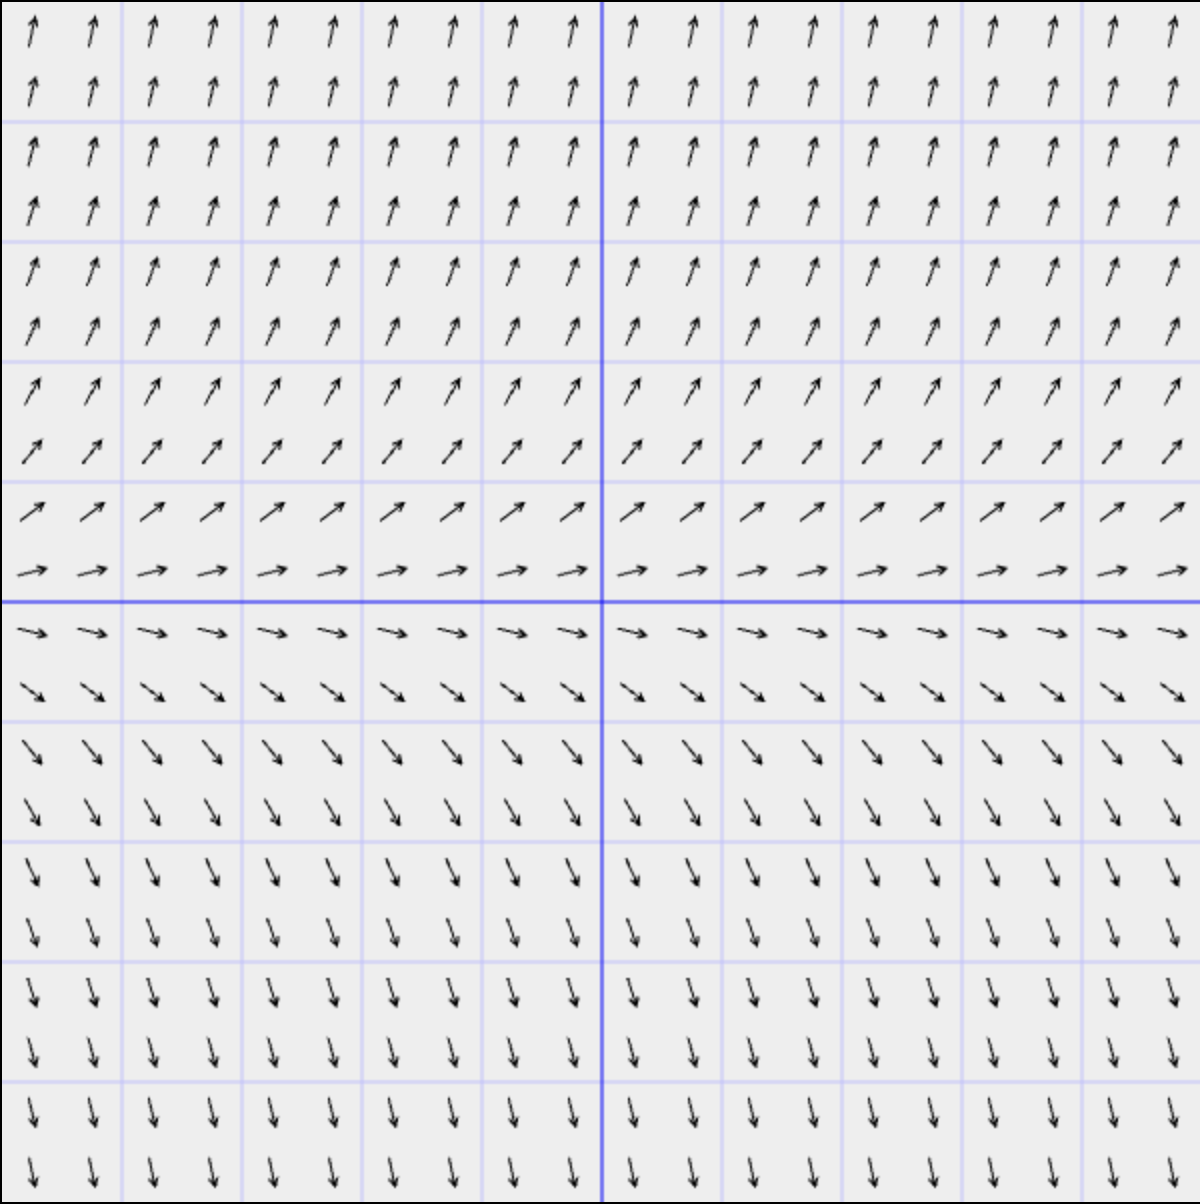
\includegraphics[width=0.45\textwidth]{Source.png}
            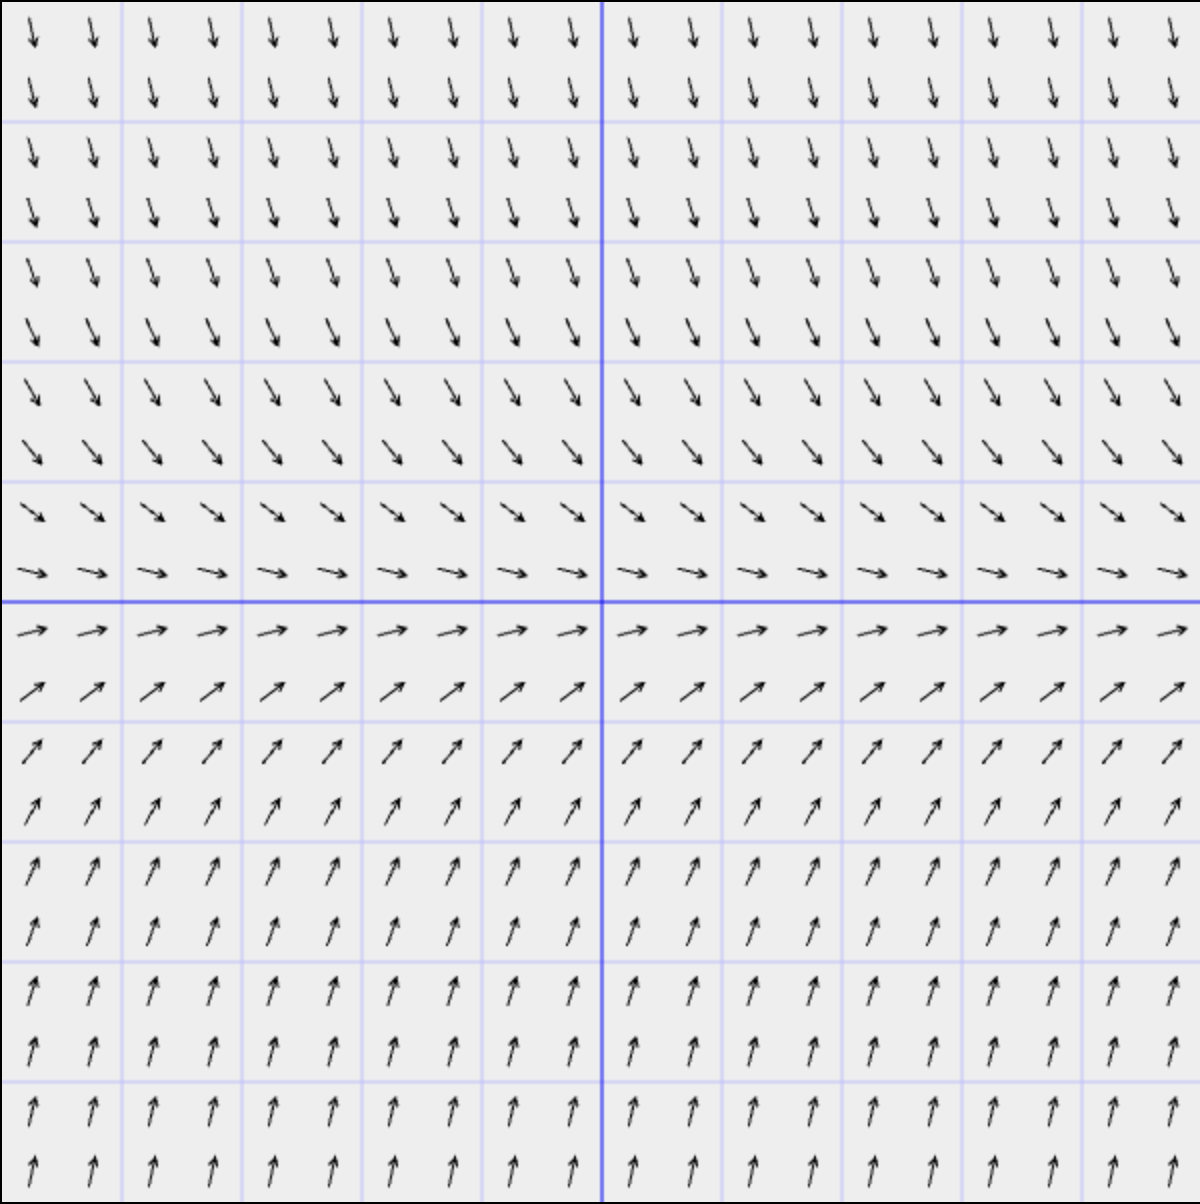
\includegraphics[width=0.45\textwidth]{Sink.png}
        \end{center}
    \end{block}
    For $a\ne 0$, the point $x=0$ is an equilibrium point.
\end{frame}

\begin{frame}{Flows}
    \begin{block}{The Flow of a Differential Equation}
        $\phi: \mathbb{R} \times \mathbb{R}^n \to \mathbb{R}^n$ is the flow of a differential equation. $\phi(t,x_0)$ is the state at time $t$ of the solution with initial condition $x_0$.
    \end{block}
    For example, the flow of the equation $x' = ax$ is given by $\phi(t,x_0) = x_0 e^{at}$. The flow is important to the Linearization Theorem, which will be discussed after more examples.
\end{frame}

\section{Systems of Differential Equations}

\begin{frame}{Systems of Differential Equations}
    A system of differential equations is a collection of $n$ differential equations of the form
    \[x_1' = f_1(t, x_1, x_2, \ldots, x_n)\]
    \[x_2' = f_2(t, x_1, x_2, \ldots, x_n)\]
    \[\vdots\]
    \[x_n' = f_n(t, x_1, x_2, \ldots, x_n)\]
    In vector form, we have
    \[
        X=
        \begin{pmatrix}
            x_1 \\
            x_2 \\
            \vdots \\
            x_n
        \end{pmatrix}
    \]
\end{frame}

\begin{frame}{Systems of Differential Equations}
    Then, the system can be expressed as
    \[
        X' = F(t, X)
    \]
    where
    \[F(t, X)=
    \begin{pmatrix}
        f_1(t, x_1, x_2, \ldots, x_n) \\
        f_2(t, x_1, x_2, \ldots, x_n) \\
        \vdots \\
        f_n(t, x_1, x_2, \ldots, x_n)
    \end{pmatrix}
    \]
    A solution of this system is then a function of the form
    \[X(t)=(x_1(t), x_2(t), \ldots, x_n(t))\]
    such that $X'(t) = F(t, X(t))$.
\end{frame}

\begin{frame}{Systems of Differential Equations}
    Consider the following system:
    \[x'=y\]
    \[y'=-x\]
    We let $x_1=x$ and $x_2=y$, so we can write this system in vector form as
    \[X'=
    \begin{pmatrix}
        x' \\
        y'
    \end{pmatrix}=
    \begin{pmatrix}
        0 & 1 \\
        -1 & 0
    \end{pmatrix}
    \begin{pmatrix}
        x \\
        y
    \end{pmatrix}
    \]
\end{frame}

\begin{frame}{Systems of Differential Equations}
    The curve $X(t)=(a\sin t, a\cos t)$ for any $a\in \mathbb{R}$ is a solution to this system, since
    \[x'(t)=a\cos t=y(t)\]
    \[y'(t)=-a\sin t=-x(t)\]
    We can look at the slope field of this system along with a few solution curves to get a better understanding of the behavior of the system.
\end{frame}

\begin{frame}{Systems of Differential Equations}
    \begin{block}{Slope Field and Solution Curves}
        \begin{center}
            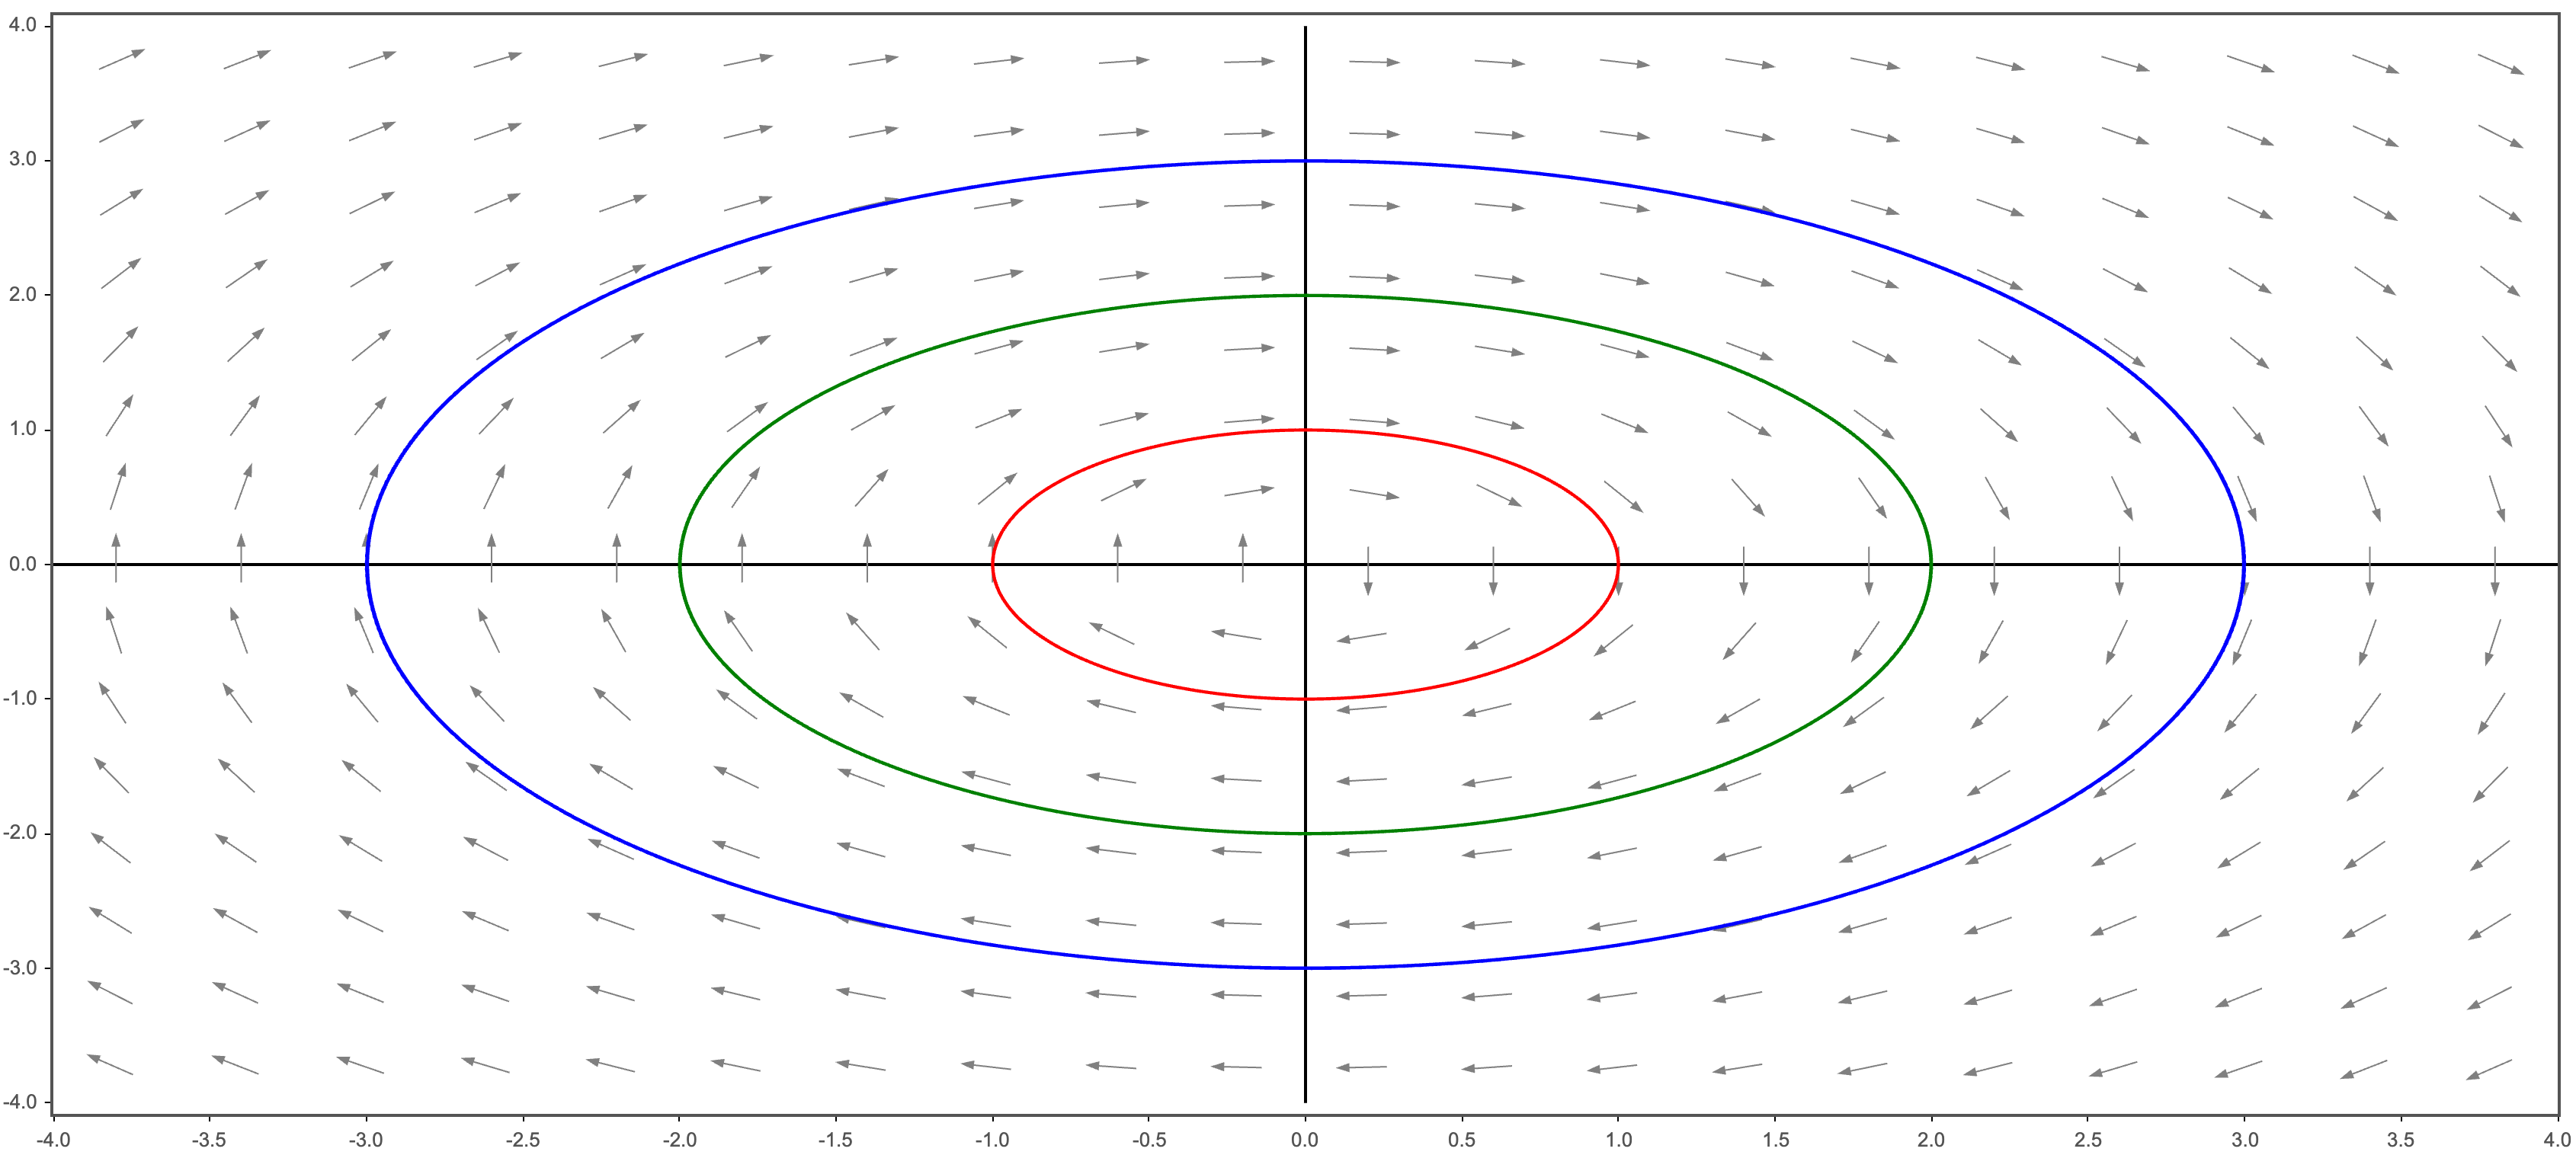
\includegraphics[width=0.9\textwidth]{HarmonicOscillator.png}
        \end{center}
    \end{block}
    As we can see from the slope field, the system describes a simple harmonic oscillator, where the solutions represent periodic motion. There are no sinks and sources in this system, but there is an equilibrium point at the origin.
\end{frame}

\begin{frame}{Definitions}
    \begin{block}{Hyperbolic Systems}
        A matrix $A$ is hyperbolic if all its eigenvalues have non-zero real parts. We also say that the system $X' = AX$ is hyperbolic if the matrix $A$ is hyperbolic.
    \end{block}
    \begin{block}{Conjugate Systems}
        Two systems $X' = AX$ and $Y' = BY$ have flows $\phi^A$ and $\phi^B$ respectively. The systems are conjugate if there exists a homeomorphism $h$ such that $\phi^B(t, h(X_0)) = h(\phi^A(t, X_0))$ for all $t$ and $X_0$. The homeomorphism $h$ is called a conjugacy, mapping the solution curves of $X'=AX$ to those of $Y'=BY$.
    \end{block}
\end{frame}

\begin{frame}{Systems of Differential Equations}
    Consider the following system:
    \[x'=x+2y\]
    \[y'=2x+y\]
    We let $x_1=x$ and $x_2=y$, so we can write this system in vector form as
    \[X'=
    \begin{pmatrix}
        x' \\
        y'
    \end{pmatrix}=
    \begin{pmatrix}
        1 & 2 \\
        2 & 1
    \end{pmatrix}
    \begin{pmatrix}
        x \\
        y
    \end{pmatrix}
    \]
    The system is hyperbolic, as the eigenvalues of the matrix $\begin{pmatrix} 1 & 2 \\ 2 & 1 \end{pmatrix}$ are $3$ and $-1$, both of which have non-zero real parts.
\end{frame}

\begin{frame}{Saddle Points}
    \begin{block}{Slope Field and Solution Curves}
        \begin{center}
            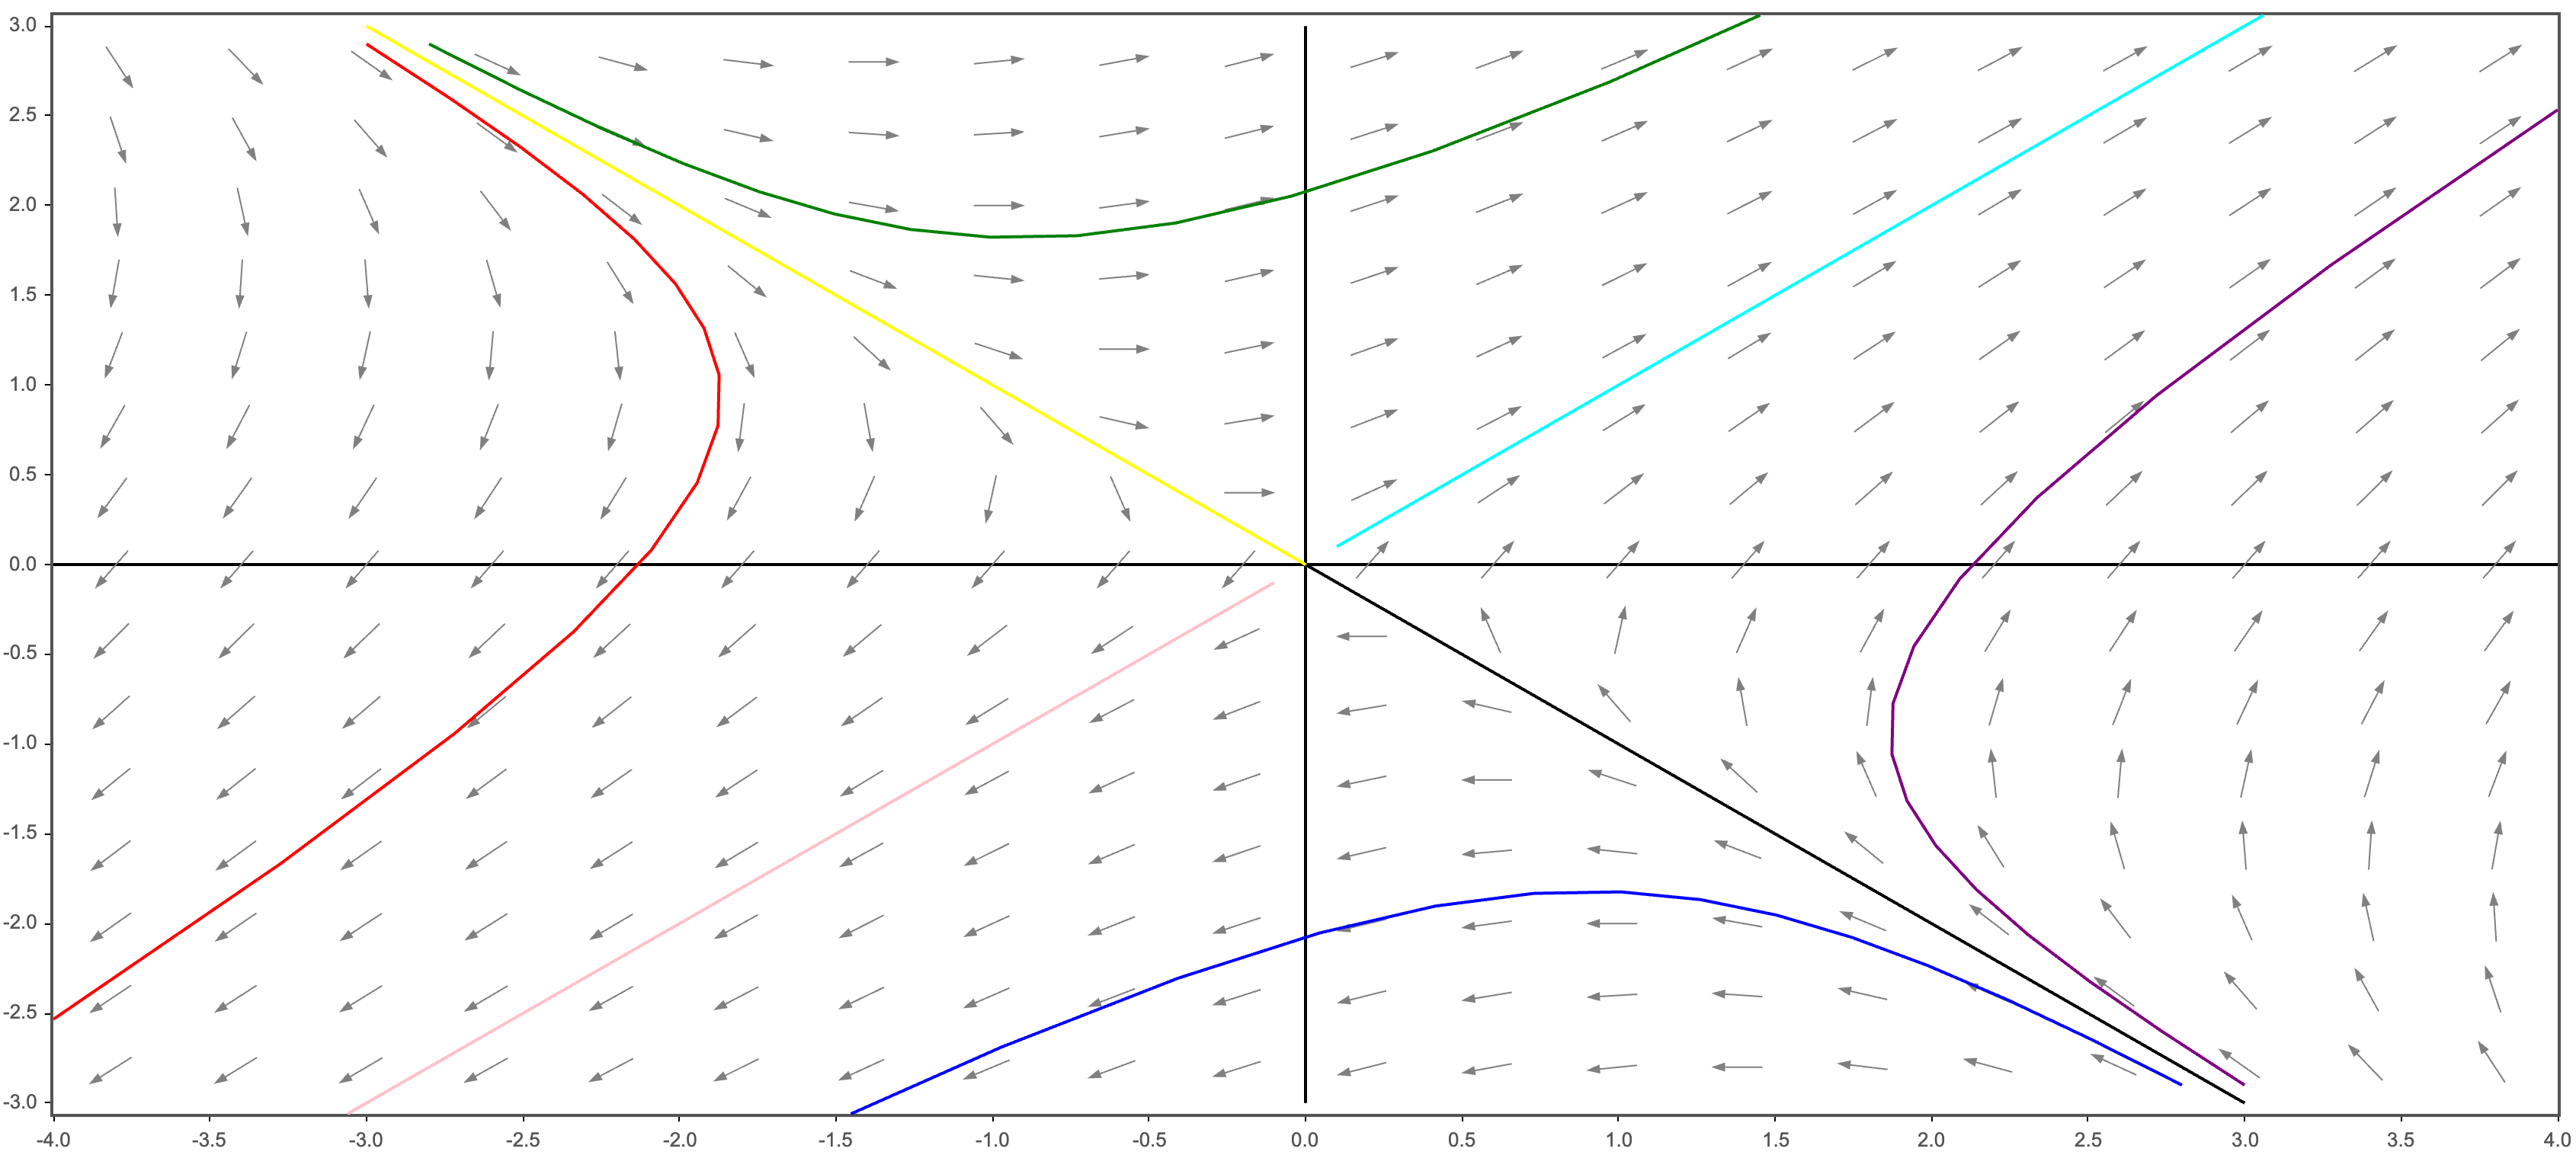
\includegraphics[width=0.7\textwidth]{Saddle.png}
        \end{center}
    \end{block}
    At the origin, there is an equilibrium point. The stable eigenspace corresponds to the eigenvalue $-1$, while the unstable eigenspace corresponds to the eigenvalue $3$. Solutions on the stable eigenspace approach the origin, but most nearby solutions eventually move away. This type of equilibrium point is called a saddle point.
\end{frame}

\section{Linearization Theorem}

\begin{frame}{Linearization Theorem}
    \begin{block}{Linearization}
        Linearization is a way to approximate a nonlinear system near an equilibrium point using its Jacobian matrix.
    \end{block}
    This idea comes from the first-order Taylor expansion: near a point, a nonlinear function can be approximated by its tangent line or tangent plane.
    \newline
    \newline
    For differential equations, this means we replace the nonlinear system with a simpler linear system that has similar behavior close to the equilibrium.
\end{frame}

\begin{frame}{Linearization Theorem}
    An equilibrium point $X^*$ is hyperbolic if the Jacobian matrix (matrix of partial derivatives) of the system evaluated at $X^*$ is hyperbolic.
    \begin{block}{Linearization Theorem}
        Suppose $X_0$ is a hyperbolic equilibrium point of the system $X' = F(X)$. Then, near $X_0$, the nonlinear flow is conjugate to the flow of the linearized system $X' = DF(X_0)X$, where $DF(X_0)$ is the Jacobian matrix of $F$ evaluated at $X_0$.
    \end{block}
\end{frame}

\begin{frame}{Linearization Example}
    Consider the nonlinear system
    \[
        x'=x+2y+x^2
    \]
    \[
        y'=2x+y+y^2.
    \]
    The origin is an equilibrium point because
    \[
        F(0,0)=(0,0).
    \]
    To understand the behavior near the origin, we linearize the system.
\end{frame}

\begin{frame}{Linearization Example}
    The Jacobian matrix is
    \[
        DF(x,y)=
        \begin{pmatrix}
            1+2x & 2 \\
            2 & 1+2y
        \end{pmatrix}.
    \]
    Evaluating at the origin,
    \[
        DF(0,0)=
        \begin{pmatrix}
            1 & 2 \\
            2 & 1
        \end{pmatrix}.
    \]
    This is the same matrix from the hyperbolic linear system we analyzed earlier. Therefore, by the Linearization Theorem, the nonlinear system is locally conjugate to the linearized system near the origin.
\end{frame}

\begin{frame}{Conclusion}
    The qualitative behavior of the nonlinear system near the origin is the same as that of the linearized system.
    \newline
    \newline
    This is powerful because nonlinear systems are generally very difficult, and often impossible, to solve explicitly.
    \newline
    \newline
    For autonomous systems near hyperbolic equilibrium points, the Linearization Theorem provides a powerful tool for understanding the dynamics.
\end{frame}

\end{document}